\section{Introducción}
\label{sec:2_marcoteorico}
Si bien el uso de robots tiene sus orígenes principalmente en fábricas para el ensamblaje de automóviles, en los últimos años la electrónica moderna ha permitido introducirlos en otras áreas, ya sea desde electrodomésticos y juguetes de la vida cotidiana, hasta viajes espaciales con el fin de explorar planetas desconocidos. Esta expansión es debido a que los mismos permiten reducir la interacción humana no solo en tareas que presentan un riesgo a la integridad de la persona, sino también en aquellas que tienen cierto grado de repetitividad.

Yendo a un caso más concreto, en el último tiempo muchas personas han adquirido los llamados robots aspiradoras, como el que se observa en la Figura \ref{fig:vaccumrobot}.a, los cuales consiguen limpiar la superficie de las casas en un tiempo medianamente razonable, aunque este tiempo no suele ser una preocupación ya que al ser el mismo completamente autónomo, uno puede seguir con sus actividades cotidianas. 

No obstante, si se analiza el recorrido que realizan la mayoría de estos robots, se puede apreciar que el mismo suele ser completamente aleatorio, y por ende se tendería a creer que no podrá pasar por toda la superficie y limpiarla completamente. La realidad es que, como están mucho tiempo circulando, logran pasar por todos los rincones de la superficie, pero esto genera que circulen más veces por unos lugares que por otros, tal como se observa en la Figura \ref{fig:vaccumrobot}.b, haciendo ineficiente el trabajo.

\begin{figure}[!ht]
    \centering
    \subfloat[Robot aspiradora comercial]{{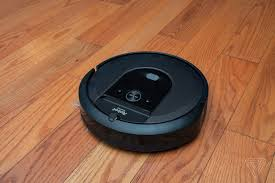
\includegraphics[width=0.47\textwidth]{Img/Roomba}}}%
    \qquad
    \subfloat[Ejemplo del recorrido de un robot aspiradora comercial]{{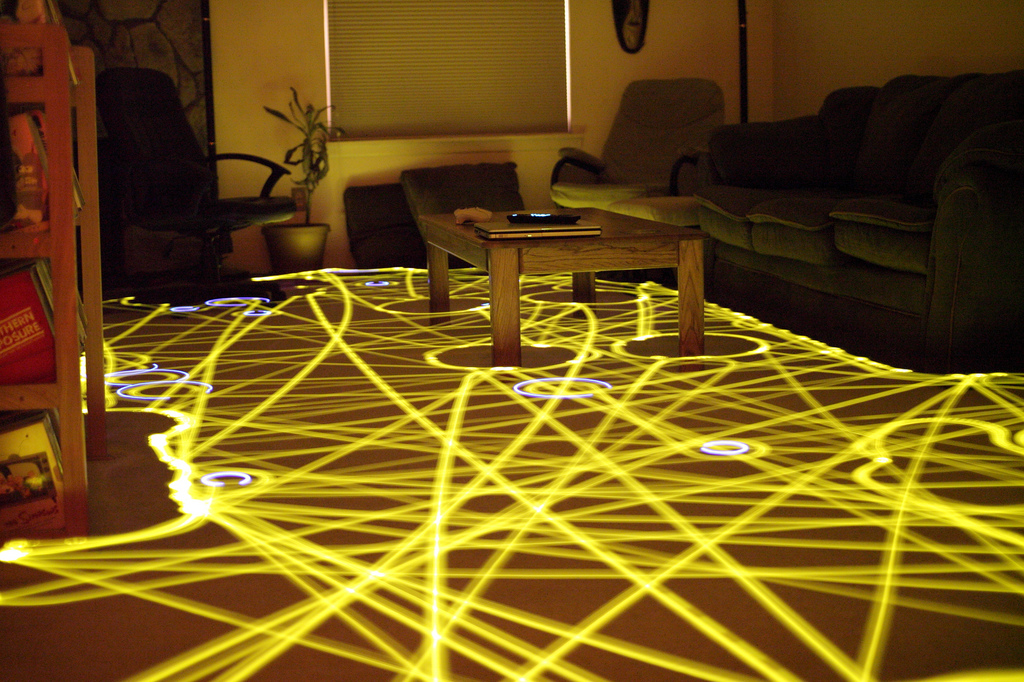
\includegraphics[width=0.47\textwidth]{Img/VaccumRobot.png}}}%
    \caption{El robot aspiradora}
    \label{fig:vaccumrobot}
\end{figure}

\ifimagenes
Si lo que se pretende es optimizar el recorrido del robot, la
\else
A pesar de que se busque reducir la interacción humana bajo estas circunstancias, no todos los robots hoy en día son autónomos, principalmente debido a la falta de robustez del algoritmo de control involucrado en el proceso. Tomando por caso el ejemplo anterior, si bien el robot aspiradora es autónomo, su eficiencia respecto a la forma óptima de realizar la tarea no es una garantía en todos los casos.

Es útil distinguir entre robots que están inmóviles, como un brazo robótico en una fábrica, y robots que son móviles, como un auto sin conductor. En este trabajo se hará hincapié en los robots móviles. Usamos este término para describir un robot impulsado por sus propios medios que puede moverse cinemáticamente entre ubicaciones en su entorno. A su vez, cuando se habla de la posición y orientación combinadas del robot, esto se define como su \textit{pose}.

Los robots móviles pueden referirse a robots que se mueven sobre el suelo, bajo el agua, a través del aire y en entornos de microgravedad, tales como los que pueden observarse en la Figura \ref{fig:mobilerobots}. Si bien este trabajo busca aplicar en parte a cualquiera de estos entornos, el enfoque del mismo se refiere principalmente a los robots móviles que permanecen en contacto con el suelo. Cada uno de ellos presentan su propia terminología para definirlos y diferenciarlos del resto, por ejemplo, el término vehículos terrestres no tripulados o UGV (del inglés \textit{unmanned ground vehicles}) a menudo se usa más específicamente para describir robots móviles terrestres, mientras que el término vehículos aéreos no tripulados o UAV (del inglés \textit{unmanned aerieal vehicles}) refieren principalmente a los drones.

Los robots móviles se mueven a través de entornos grandes y potencialmente dinámicos, lo que hace que la percepción sea mucho más difícil que los robots industriales con entornos de trabajo limitados y parámetros operativos rígidos. Por lo tanto, los robots móviles requieren sensores adicionales, una mejor percepción y mayores grados de autonomía para operar en entornos del mundo real que cambian con frecuencia.


\begin{figure}%
    \centering
    \subfloat[Wheeled robot]{{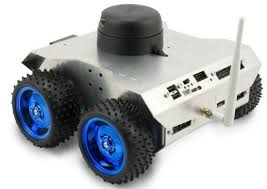
\includegraphics[width=0.25\linewidth]{Img/WheeledRobot.jpeg}}}%
    \qquad
    \subfloat[Legged robot]{{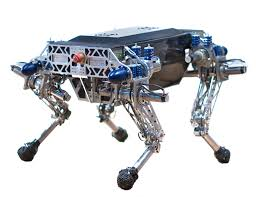
\includegraphics[width=0.25\linewidth]{Img/LeggedRobot.jpeg}}}%
    \qquad
    \subfloat[Tracked robot]{{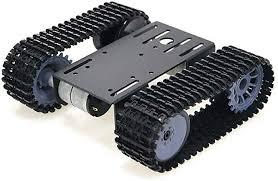
\includegraphics[width=0.25\linewidth]{Img/TrackedRobot.jpeg}}}%
    \qquad
    \subfloat[Drone]{{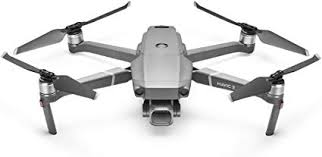
\includegraphics[width=0.3\linewidth]{Img/Drone.jpeg}}}%
    \qquad
    \subfloat[Water-based robot]{{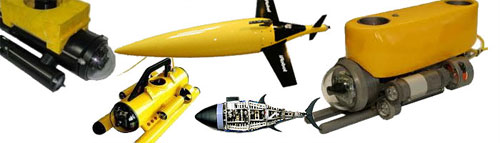
\includegraphics[width=0.5\linewidth]{Img/WaterBasedRobot.jpg}}}%
    \caption{Tipos de robot móviles}
    \label{fig:mobilerobots}
\end{figure}

Dentro de lo que respecta a robótica móvil, uno de sus desafíos actuales es lograr la completa autonomía del vehículo. Una gran parte de las empresas de la industria automotriz han dedicado mucho tiempo y dinero para lograr el objetivo. La investigación ha avanzado hasta el punto de que en la actualidad hay autos semi-autónomos disponibles en el mercado, y se cree ampliamente que en el futuro cercano casi todos los vehículos serán completamente autónomos. Para lograr esto, obviamente hay una necesidad de sensores y funciones avanzadas. Uno de los principales problemas es el hecho de que el vehículo debe ser consciente de su posición actual dentro de un entorno desconocido. Este proceso de determinar no solo su posición, sino también el mapa que lo rodea se conoce como la \textit{localización y mapeo simultáneos}, comúnmente abreviado como \textit{SLAM} (del inglés, \textit{simultaneous localization and mapping}).

El SLAM es un problema difícil de solucionar, así como lo fue para los humanos en el pasado. Tiempo atrás, los marineros usaban los llamados registros de fichas para estimar su velocidad y extrapolaban esta velocidad con el tiempo para calcular su pose. Este proceso de navegación por estima (en inglés, \textit{dead reckoning}) conduce inevitablemente a errores graves de posicionamiento con el tiempo y, por lo tanto, siempre se ha respaldado mediante el uso de puntos de referencia (o \textit{landmarks}) para la navegación. Quedándonos en este caso particular, con el uso de las estrellas los marineros lograban saber donde estaba el Norte, permitiendo corregir su dirección. Sin embargo, no siempre se podía observar este patrón por días debido al cielo nublado, entonces tenían que confiar solamente en su navegación por estima, haciendo que la incertidumbre crezca día tras día. Para el caso de los robots, cuando el mismo recorre un mapa completamente desconocido, acumulará error debido a las predicciones que debe tomar respecto a su pose y entorno en el que está, hasta el momento en que entra a un área con puntos de referencia conocidos, pudiendo así corregir su estimación de posición.

Volviendo al ejemplo del robot de limpieza, si el mismo conociera el mapa en el que se encuentra, podría entonces trazar la ruta mas óptima para realizar la limpieza del lugar. Como no todos los ambientes son iguales y cada uno tiene, por ejemplo, muebles ubicados en distintos lugares, dicho robot podría hacer primero un reconocimiento del lugar previo a la limpieza para tener una noción de todo el espacio, o bien obtener el mapa y la ubicación en la que se encuentra en base al movimiento que realiza, pasando por los lugares que le faltaron aspirar. Para cualquiera de las dos opciones, por lo tanto, necesitará tanto tomar los datos del lugar como controlar al vehículo para que vaya circulando por el ambiente.

La
\fi
estimación de la pose, entonces, es una parte no separable de aplicaciones como el control del vehículo y el mapeo. Varios sensores se utilizan comúnmente para estimar la pose de un robot. Las unidades de medición inercial (IMU), la cámara, la odometría de las ruedas\footnote{Se mide la rotación de las ruedas para estimar cambios de la posición del vehículo a lo largo del tiempo} para el caso de ciertos robots móviles y el LiDAR se encuentran entre los sensores más populares para la localización en interiores \cite{delrosario2016}, mientras que para exteriores suele sumarse el GPS a estos sensores, corrigiendo al mismo mediante acción de la IMU \cite{caron2006}.


\ifimagenes
\else
En la localización al aire libre, la señal del sistema de posicionamiento global (GPS) suele estar disponible y, dado que la posición se puede obtener con precisión mediante GPS, es la opción común para la fusión con los datos obtenidos de la IMU \cite{engel2014}. Sin embargo, en un entorno denegado por GPS, como dentro de un edificio, se deben usar otros sensores para corregir las estimaciones de la IMU. Un enfoque común para abordar este problema son la fusión IMU-cámara \cite{mirzaei2008}, \cite{hesch2009}, \cite{chambers2014}, \cite{hesch2013}, así como también el uso de LiDAR \cite{lee2016}.

Un algoritmo SLAM robusto es esencial para que cualquier robot móvil navegue de manera segura a través de un entorno no estructurado. El algoritmo SLAM con frecuencia define un marco de coordenadas global para que el robot opere; uno que generalmente es utilizado por todas las funcionalidades de alto nivel, como navegación, planificación de rutas, exploración, identificación de objetos, seguimiento de objetos y manipulación de los mismos. Estas dependencias hacen que el algoritmo SLAM sea una parte central de cualquier arquitectura de robot móvil, y las fallas irrecuperables son altamente indeseables. Es probable que cualquier robot desorientado por una falla de SLAM no pueda realizar su tarea, o peor, puede poner en peligro a los humanos, a sí mismo o al medio ambiente.

%Si bien se han demostrado varios algoritmos SLAM en laboratorios, es más difícil producir soluciones robustas en entornos no estructurados del mundo real. El deslizamiento de las ruedas, por ejemplo, puede producir mediciones de odometría ruidosas, mientras que los sensores del sistema de posicionamiento global (GPS) a menudo producen una localización global con saltos muy pronunciados para la misma posición. El SLAM robusto del mundo real se vuelve aún más difícil cuando estos errores de detección aleatorios y sistemáticos ocurren en entornos que tienen geometrías redundantes u objetos en movimiento. Por ejemplo, en el caso de los LIDAR bidimensionales, los algoritmos empleados con los mismos suelen presuponer que el robot se encuentra terrestre se encuentra sobre una superficie plana, tal como puede ser el cuarto de un hogar. Si la superficie presenta irregularidades muy marcadas, la tarea de mapeo en dos dimensiones del mismo aumentaría su complejidad, ya que no podría encontrar las relaciones entre los datos anteriores con los actuales (no coincidirían) por si solo, y dependería de sensores adicionales, como una IMU.

%Para poder realizar las tareas en tiempo real, es necesario contar con una capacidad de cómputo suficiente para no sólo adquirir todos los datos de los sensores, sino también procesarlos para conseguir el mapa junto a la pose en cada momento. En el presente trabajo, se desarrolla una plataforma de Hardware capaz de realizar dicha actividad, a su vez de describir dos algoritmos de SLAM, uno basado en la combinación de un LIDAR 2D junto a una IMU, y el otro basado en una cámara RGB-D, obteniendo entonces un SLAM tridimensional.
\fi



En particular, para el caso de la localización y mapeo tridimensional (SLAM 3D), los LIDAR 3D han adquirido bastante popularidad en el último tiempo con la llegada de los vehículos autónomos, aunque son muy costosos. Si se pretende entonces una opción más económica, las cámaras estéreo y RGB-D (\textit{D: Depth - profundidad}) son de las más utilizadas para esto, a su vez de poder obtener datos de color de las mismas. Los sensores RGB-D como la \textit{Microsoft Kinect} proporcionan directamente mapas de profundidad densos e imágenes en color. En general, los enfoques SLAM que operan en imágenes RGB-D son estructuralmente diferentes de los sistemas estéreo, ya que la entrada es RGB-D de profundidad en lugar de dos imágenes de color. A pesar de esto, pueden obtenerse nubes de puntos de profundidad a partir de ambos sensores con el procesamiento
\ifimagenes
\ifimagenespaper
adecuado, como los presentados por la librería OpenCV \cite{kaehler2017}.
\else
adecuado, lo cual se desarrolla en el apéndice.
\fi
\else
adecuado, como los presentados por la librería OpenCV \cite{kaehler2017}.
\fi

Una vez obtenidas las nubes de puntos de profundidad, una de las formas de calcular la posición y orientación del robot (conocido como la \textit{pose} del robot) a lo largo del tiempo es mediante la comparación entre dos nubes de puntos contiguas (una con los datos recientes y otra con los datos de la nube de puntos anterior), buscando en definitiva la transformación necesaria para que la nube de puntos actual pueda alinearse (o sea, que coincida lo mejor posible) con la nube de puntos anterior. Este proceso se lo conoce como el \textit{registro de la nube de puntos}, y suele llevar una serie de pasos, lo cual se desarrollará más adelante. Para poder facilitar el uso de nubes de puntos, existen librerías específicas para trabajar con dicha información, siendo algunas de ellas la \textit{Point Cloud Library} y \textit{Open3D}, las cuales implementan no sólo distintos algoritmos, sino también estructuras para facilitar el manejo de las nubes de puntos.

Si bien hay muchos robots móviles hoy en día en el mercado, gran parte de ellos son costosos, y sobre todo los que se encuentran equipados para realizar SLAM 3D. Para poder evaluar los algoritmos necesarios sin tener que ponerse en gasto, existen entornos de simulación pensados, entre otras cosas, para robots, consiguiendo resultados símiles a la realidad. Unos de los más conocidos en el ámbito son \textit{V-REP} y \textit{Gazebo}, siendo este último el elegido para realizar el trabajo.

\subsection{Contribuciones}
En el presente trabajo, 
\ifimagenes
se desarrolla un algoritmo de registro de nube de puntos en base a los datos obtenidos de una cámara RGB-D en movimiento dentro de un ambiente estático, bajo el entorno de simulación Gazebo. En base a la transformación obtenida en cada iteración, se aplica la misma a la nube de puntos entrante, para luego sumarla al mapa 3D generado.

Como el trabajo presentado forma parte de una tesis de grado en desarrollo sobre SLAM 2D y 3D, se pretende que el mismo pueda fusionarse con los datos provenientes de otros sensores, en particular la IMU y el LIDAR 2D, para obtener una mejor estimación de la posición y, por consiguiente, obtener un mapa más exacto.

\else
se presenta una plataforma de Hardware capaz de realizar las tareas de SLAM que incluyen una gran cantidad de sensores, a su vez de contar la misma con un factor de forma de Hardware para que la misma pueda expandir sus funcionalidades en base a lo que requiera el usuario.

Luego, e describen dos algoritmos de SLAM, uno basado en la combinación de un LIDAR 2D junto a una IMU, y el otro basado en una cámara RGB-D, obteniendo entonces un SLAM tridimensional, ambos considerando un entorno estático. Debido a la falta de sensores capaces de brindar la información reuqerida, se realizaron las pruebas del mismo bajo el entorno de simulación Gazebo, con el fin de poder luego llevarlas a un escenario real cuando se tenga el robot completo.
\fi

A su vez, se provee de un código compatible con \textit{ROS}, un framework pensado para utilizar en robótica, permitiendo portabilidad y versatilidad a la hora de proporcionar los datos de los sensores, ya que el mismo utiliza un sistema de mensajes que permite vincular a dos procesos sin importar el método de adquisición o procesamiento de los datos, mientras los mismos respeten el tipo de mensaje en sí.

\subsection{Estructura del documento}
El presente documento se compone de las siguientes secciones
\ifimagenespaper
\else
y apéndices
\fi
\begin{itemize}
    \item \textbf{Introducción}: esta sección hace una breve introducción al SLAM, presentando los distintos sensores utilizados normalmente, a su vez de dar una primera aproximación al registro de nubes de puntos con los sensores RGB-D para realizar dicha tarea. A su vez, se mencionan las contribuciones realizadas.
    \ifimagenespaper
    \item \textbf{Marco teórico}:
    \else
    \item \textbf{Herramientas para el desarrollo de robots}: En esta sección se da una introducción al framework \textit{ROS}, en particular a su estructura y su modo de vinculación entre los distintos paquetes. Finalmente, se da una breve descripción de Gazebo.
        \ifimagenes
    \item \textbf{Marco teórico}:
        \else
    \item \textbf{Geometría tridimensional y marcos de referencia}: en esta sección se desarrollan los conceptos de la geometría tridimensional necesarias para abordar los temas del trabajo realizado, a su vez de mencionar distintos marcos de referencia usualmente utilizados.
    \item \textbf{Análisis de regresión}: en esta sección se desarrolla el denominado análisis de regresión, abarcando tanto la regresión lineal como la no lineal.
    \item \textbf{Estimación de estado}: siguiendo con el análisis de regresión, en esta sección se desarrollan distintos algoritmos de estimación de estado, siendo uno de los mas conocidos el filtro de Kalman.
    \item \textbf{Sensores}: en esta sección se mencionan distintos sensores utilizados comúnmente en lo que refiere al SLAM, a su vez de presentar distintos métodos de calibración de algunos de ellos y características importantes.
    \item \textbf{Simultaneous Localization And Mapping}: en esta sección se profundiza en lo que refiere al SLAM, mencionando no sólo distintos algoritmos que existen, sino también mencionando características importantes de la técnica en si.
    \item \textbf{Reconstrucción del entorno}:
        \fi
    \fi 
    en esta sección se describe tanto el flujo de trabajo del registro de nubes de puntos asi como también los distintos algoritmos utilizados comúnmente a la hora de realizarlo, asociando a los mismos con su implementación en la librería PCL. A su vez, se comenta como conseguir las nubes de puntos en base a los sensores utilizados comúnmente en este tipo de
    \ifimagenes
    aplicaciones, además de una calibración de los mismos.
    \item \textbf{Experimentos}: En base a la sección anterior, en esta se describe el flujo del algoritmo realizado, además de presentar los resultados obtenidos en base a la simulación realizada
    \else
    aplicaciones.
    \item \textbf{Plataformas disponibles}: en base a los sensores y datos necesarios, en esta sección se realiza un relevamiento de las distintas plataformas disponibles en el mercado, comparando cada una de ellas.
    \item \textbf{Resolución}: en esta sección se mencionan los métodos utilizados para lograr el objetivo del trabajo, basándose en las secciones anteriores. A su vez, se muestran los resultados obtenidos.
    \fi
    \item \textbf{Conclusiones}: En esta sección se desarrolla la finalidad conseguida del trabajo, evaluando distintos puntos de interés.
    \ifimagenes
    \item \textbf{Trabajos futuros}: en esta sección se mencionan distintos aspectos para lo que sigue luego de este trabajo.
    \else
    \item \textbf{Apéndices}: en esta sección se incluye información útil, como el esquemático de la placa realizada.
        \ifimagenespaper
        \else
    \item \textbf{Anexo}: Finalmente, se incluye un anexo con información útil a la hora de querer llevar a cabo una implementación con sensores físicos, utilizando los datos proporcionados por los mismos.
        \fi
    \fi
\end{itemize}